%The \ssww upgrade study is a good opportunity to try to optimize the signal event selection.
The default event selection is optimized in order to improve the strength of the \ssww EWK signal.
The expectation is that the increased detector acceptance from the forward tracking combined with an increase in center of mass energy and much higher integrated luminosity will allow tighter selection cuts without jeopardizing signal statistics.

%------------------------------------------------------------------------------------------------------
%
%------------------------------------------------------------------------------------------------------
\subsection{Random grid search algorithm}\label{sswwupgrade:opt_rgs}
The chosen method for optimizing the event selection is a cut-based algorithm known as the Random Grid Search (RGS) \cite{2018.rgs-paper}.
Consider a simple case of two variables $x$ and $y$ chosen to differentiate signal from background.
In order to be considered a signal event, a given event would be required to pass a set of selection criteria, called a \emph{cut point}: $c = \{x > x_c, y > y_c\}$.
A simple method to choose the optimal cut point (i.e. the ``best'' values of the cuts $x_c$ and $y_c$) would be to construct an $n\times m$ rectangular grid in $x$ and $y$ consisting of points $(x_0,y_0), (x_1,y_1), ..., (x_n,y_m)$, as Figure~\ref{fig:rgs_grids_rectangular}.
One can then choose a cut point $c_k = \{x > x_i, y > y_j\}$ that maximizes the signal significance as given by a chosen metric.
This would be considered a \emph{rectangular grid search}.

While effective in principle, a rectangular grid search comes with two major drawbacks:
\begin{enumerate}
\item The algorithm scales exponentially as the number of variables to be optimized increases, as this is effectively increasing the dimensionality of the grid.  In the simple case of a square grid with $N$ bins per variable $v$, the number of cut points to be evaluated grows as $N^v$.
\item Signal and background samples are rarely evenly distributed over the entire grid, resulting in many cut points being sub-optimal and evaluating them would be a waste of computing resources.
\end{enumerate}

To combat these limitations, the RGS algorithm constructs a grid of cut points directly from the signal sample itself.
In the two-dimensional example, this means that the variables $x_i$ and $y_j$ making up the cut point $c_k = \{x > x_i, y > y_j\}$ take their values directly from a given signal event.
This has the benefit of creating a \emph{random grid} of cut points that is biased towards regions of high signal concentration by construction.
This reduces the need for exponentially increasing numbers of cut points while ensuring that computing resources are not wasted in regions with few to no signal events.
An example of a two-dimensional random grid is shown in Figure~\ref{fig:rgs_grids_random}.

\begin{figure}[htp]
  \centering
  \begin{subfigure}[b]{.48\textwidth}
    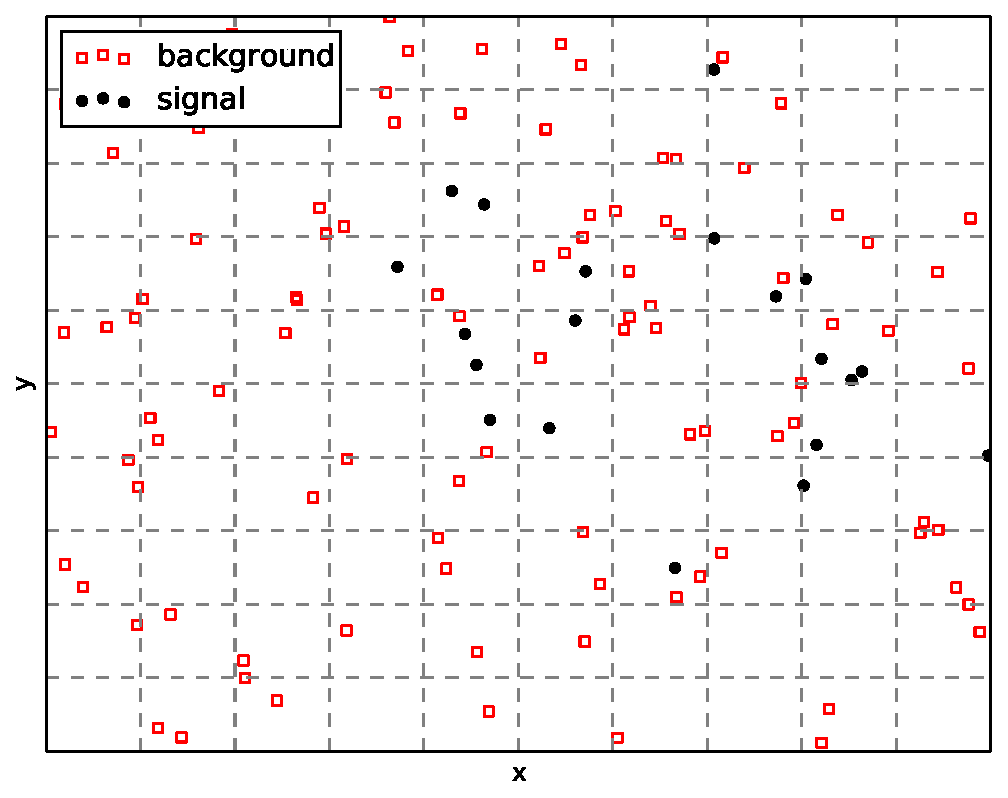
\includegraphics[width=\textwidth]{figs/ssww_upgrade/rgs/square_grid-cropped}
    \caption{Rectangular grid}
    \label{fig:rgs_grids_rectangular}
  \end{subfigure}
  \begin{subfigure}[b]{.48\textwidth}
    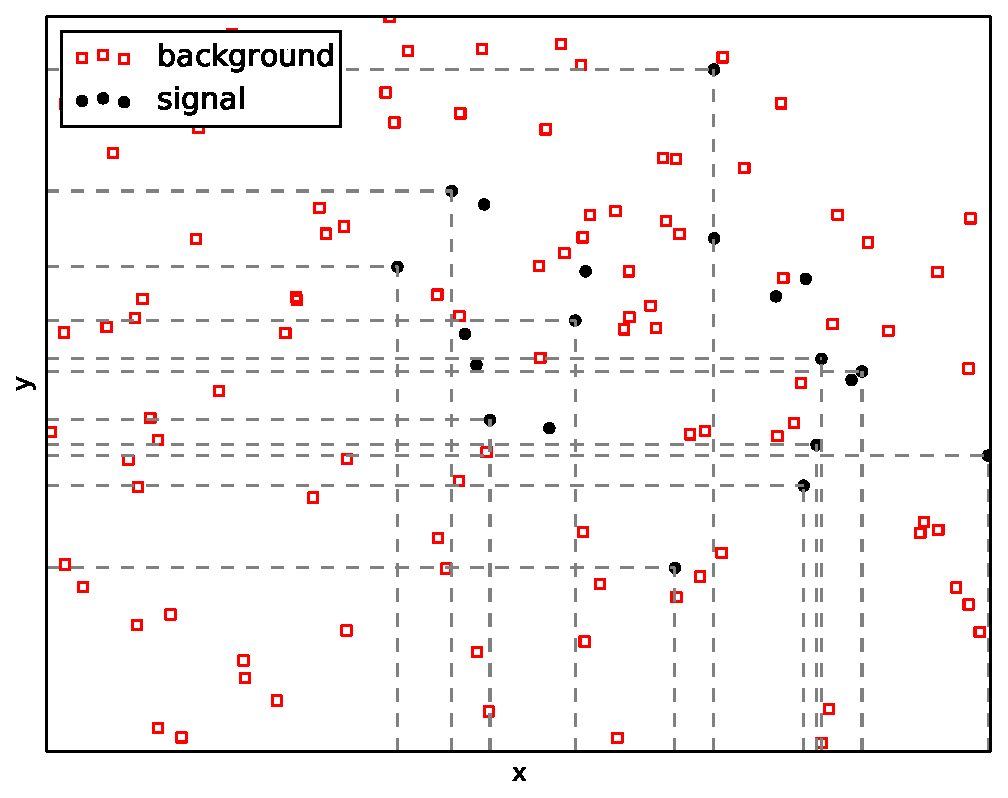
\includegraphics[width=\textwidth]{figs/ssww_upgrade/rgs/random_grid-cropped}
    \caption{Random grid}
    \label{fig:rgs_grids_random}
  \end{subfigure}
  \caption{A visual representation of a two-dimensional rectangular grid (left) and a random grid (right) in variables $x$ and $y$.  The signal events are the black circles, and the red squares are the background events.  Each intersection of gray dashed lines represents a cut point to be evaluated by the optimization.}
  \label{fig:rgs_grids}
\end{figure}

Once the random grid of cut points is constructed, the optimal cut point can be chosen using any number of metrics, such as signal to background ratio.
For the purpose of the \ssww upgrade study, the optimal cut point is chosen to be the one that mazimizes the signal significance $Z$ as defined in Equation~\ref{eq:significance_with_error} \cite{2011.asimov-significance}:
\begin{equation}
Z = \sqrt{2{\bigg[}(s+b)\ln{\Big(}\frac{s+b}{b_0}{\Big)}+b_0-s-b{\bigg]}+\frac{(b-b_0)^2}{\sigma_b^2}}
\label{eq:significance_with_error}
\end{equation}
where $s$ and $b$ are the number of signal and background events, respectively, $\sigma_b$ is the total uncertainty on the background, and $b_0$ is defined as:
\begin{equation}
b_0 = \frac{1}{2}{\Big(}b-\sigma_b^2+\sqrt{(b-\sigma_b^2)^2+4(s+b)\sigma_b^2}{\Big)}
\label{eq:significance_b0}
\end{equation}

In the case where the backround is known precisely (i.e. $\sigma_b = 0$), Equation~\ref{eq:significance_with_error} simplifies to
\begin{equation}
Z = \sqrt{2\bigg(b\big[(1+s/b)\ln(1+s/b)-s/b\big]\bigg)}
\label{eq:significance_without_error}
\end{equation}
which further reduces to the familiar $Z = s/\sqrt{b}$ for the case when $s << b$.

%------------------------------------------------------------------------------------------------------
%
%------------------------------------------------------------------------------------------------------
\subsection{Inputs to the optimization}\label{sswwupgrade:opt_inputs}
In order to train the RGS, signal and background samples are prepared from events passing the event selection outlined in Table~\ref{tab:sswwupgrade_event_selection} up through the $b$-jet veto.
The signal sample is chosen to be the longitudinally polarized \ssww EWK events, and the transverse and mixed polarizations are treated as background along with \ssww events from QCD interactions and the traditional backgrounds listed in Section~\ref{sswwupgrade:background}.
Splitting the inclusive \ssww EWK events by polarization allows the optimization to favor the longitunally polarized events as much as possible, even though they both contribute to the EWK signal.

The following variables are chosen for optimization:
\begin{itemize}
\item Leading lepton $\pt$
\item Dilepton invariant mass ($\mll$)
\item Leading and subleading jet $\pt$
\item Dijet invariant mass ($\mjj$)
\item Lepton-jet centrality ($\zeta$)
\end{itemize}
Subleading lepton $\pt$ is omitted as it is desirable to keep the cut value as low as possible due to its sensitivity to the longitudinal polarization (as discussed in Section~\ref{sec:sswwupgrade_longitudinal_sens}); despite this, the leading lepton $\pt$ is still allowed to be optimized as it can have strong background rejection power.
Additionally, the dijet separation $\detajj$ was included in early studies of the optimization, however it was dropped due to the cut value being motivated by well-studied differences between EWK- and QCD-produced \ssww events (as in Figure~\ref{fig:ssww13tev_dijet_comparison_dyjj}).

Two additional constraints were imposed when selecting the optimal cut point:
\begin{enumerate}
\item At least 1000 signal events must survive in order to prevent the optimization from being too aggressive and unnecssarily reducing signal statistics.
\item The dijet invariant mass may only vary within a $50\gev$ range of the default value (from $450-550\gev$) due to the cut being physically motivated by the VBS event topology described in Section~\ref{ssww13tev:ssww_topology}.
\end{enumerate}

Lastly, the signal significance is calculated without taking into account the uncertainty of the background using Equation~\ref{eq:significance_without_error}.
This is due to the fact that the statistical uncertainties of the fake electron and charge misidentification backgrounds are quite large, owing to poor MC statiscs in a few of the samples.
If Equation~\ref{eq:significance_with_error} were used instead, the optimization would cut unreasonably hard against these backgrounds.
Since Monte Carlo statistics is not expected to be a limiting factor when this analysis is performed at the HL-LHC, it is more realistic to simply ignore these large statistical uncertainties for the purpose of the optimization.

%------------------------------------------------------------------------------------------------------
%
%------------------------------------------------------------------------------------------------------
\subsection{Results of the optimization}\label{sswwupgrade:opt_results}
Ultimately, the random grid is constructed from over 38,000 LL-polarized \ssww events in the six variables listed above.
After applying the constraints, the optimal cut point reduces the total background from 9900 to 2310 while reducing the signal from 3489 to 2958.
This corresponds to an increase in signal significance from $Z = 33.26$ to $Z = 52.63$ as calculated by Equation~\ref{eq:significance_without_error}.
The updates to the event selection are listed in Table~\ref{tab:sswwupgrade_optimized_selection}. %, and plots of the optimized variables are found in Figures~\ref{fig:optimized_lep0pt}-\ref{fig:optimized_centrality}.

The large reduction in the background is primarily a result of increasing the leading and subleading jet $\pt$ from $30\gev$ to $90\gev$ and $45\gev$, respectively.
As can be seen in Figure~\ref{fig:optimized_jetpt}, this increase removes a significant portion of the backgrounds from jets faking electrons and charge mis-ID.
Additionally, the loosening of the lepton-jet centrality cut $\zeta$ allows more signal events to survive the event selection (see Figure~\ref{fig:optimized_centrality}).
Other changes to the event selection are minor and do not individually have a large impact on the signal or background yields; similar distributions of these variables are shown in Appendix~\ref{app:sswwupgrade_optimization_plots}.

The full event yields after optimization as well as the cross section measurement are detailed alongside those using the default selection in Section~\ref{sswwupgrade:results}.

\begin{table}[htb]
  \centering
  \begin{tabular}{l|c}
    Selection requirement              & Selection value \\
    \hline\hline
    Lepton kinematics                  & $\pt > 28\gev$ (leading lepton only) \\
    %                                   & $\pt > 25\gev$ (subleading lepton) \\
    \multirow{2}{*}{Jet kinematics}    & $\pt > 90\gev$ (leading jet) \\
                                       & $\pt > 45\gev$ (subleading jet) \\
    \hline
    %Dilepton charge                    & Exactly two signal leptons with same charge\\
    %Dilepton separation                & $\Delta R_{l,l} \ge 0.3$ \\
    Dilepton mass                      & $m_{ll} > 28\gev$ \\
    %$Z$ boson veto                     & $|m_{ee} - m_Z| > 10\gev$ ($ee$-channel only) \\
    %$\met$                             & $\met > 40\gev$ \\
    %Jet selection                      & At least two jets with $\Delta R_{l,j} > 0.3$\\
    %$b$ jet veto                       & $N_{\textrm{b-jet}} = 0$\\
    %Dijet separation                   & $\Delta\eta_{j,j} > 2.5$\\
    %Trilepton veto                     & No additional preselected leptons\\
    Dijet mass                         & $m_{jj} > 520\gev$ \\
    Lepton-jet centrality              & $\zeta > -0.5$ \\
    \hline
  \end{tabular}
  \caption{Updates to the \ssww event selection criteria after optimization.  Cuts not listed remain unchanged from the default selection in Table~\ref{tab:sswwupgrade_event_selection}.}
  \label{tab:sswwupgrade_optimized_selection}
\end{table}

\begin{figure}[htp]
  \centering
  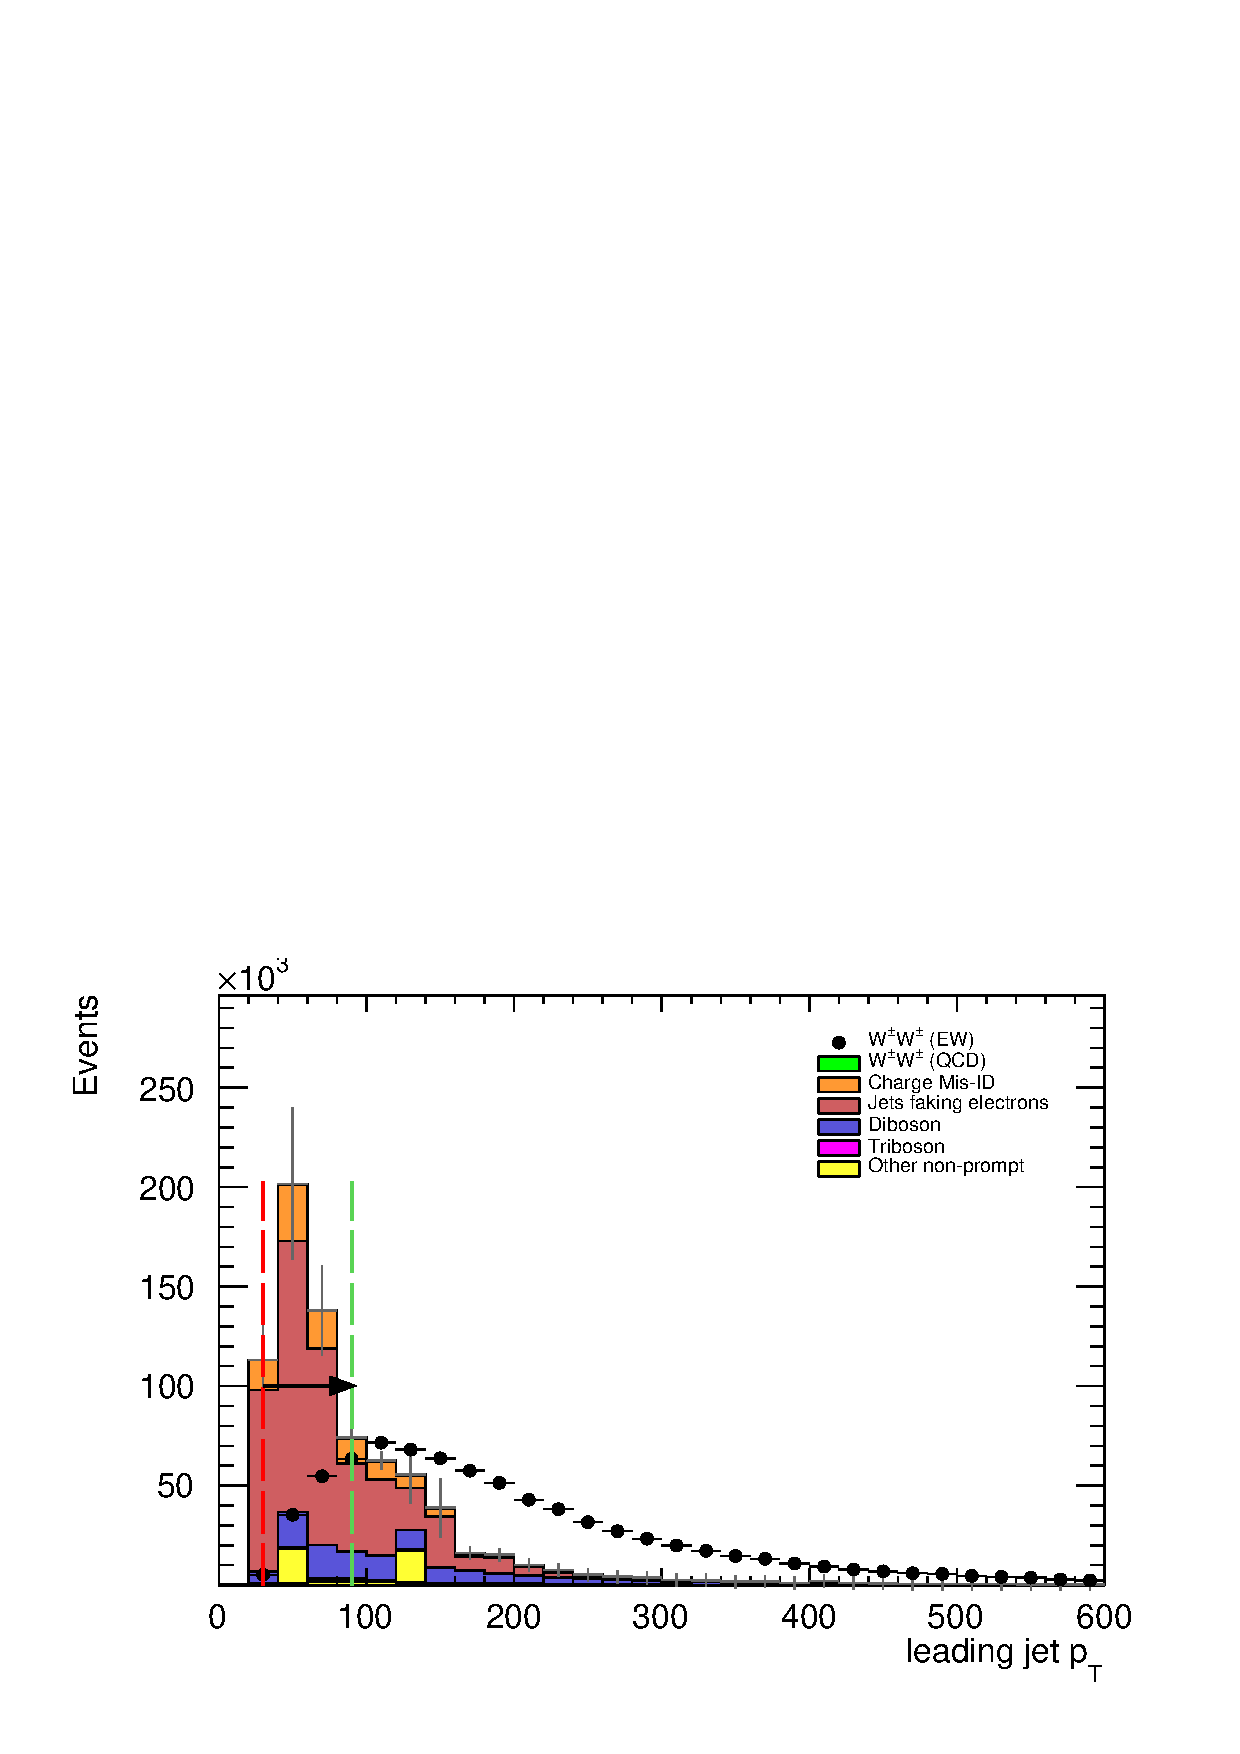
\includegraphics[width=0.6\textwidth]{figs/ssww_upgrade/optimization_plots/jet0pt}\\
  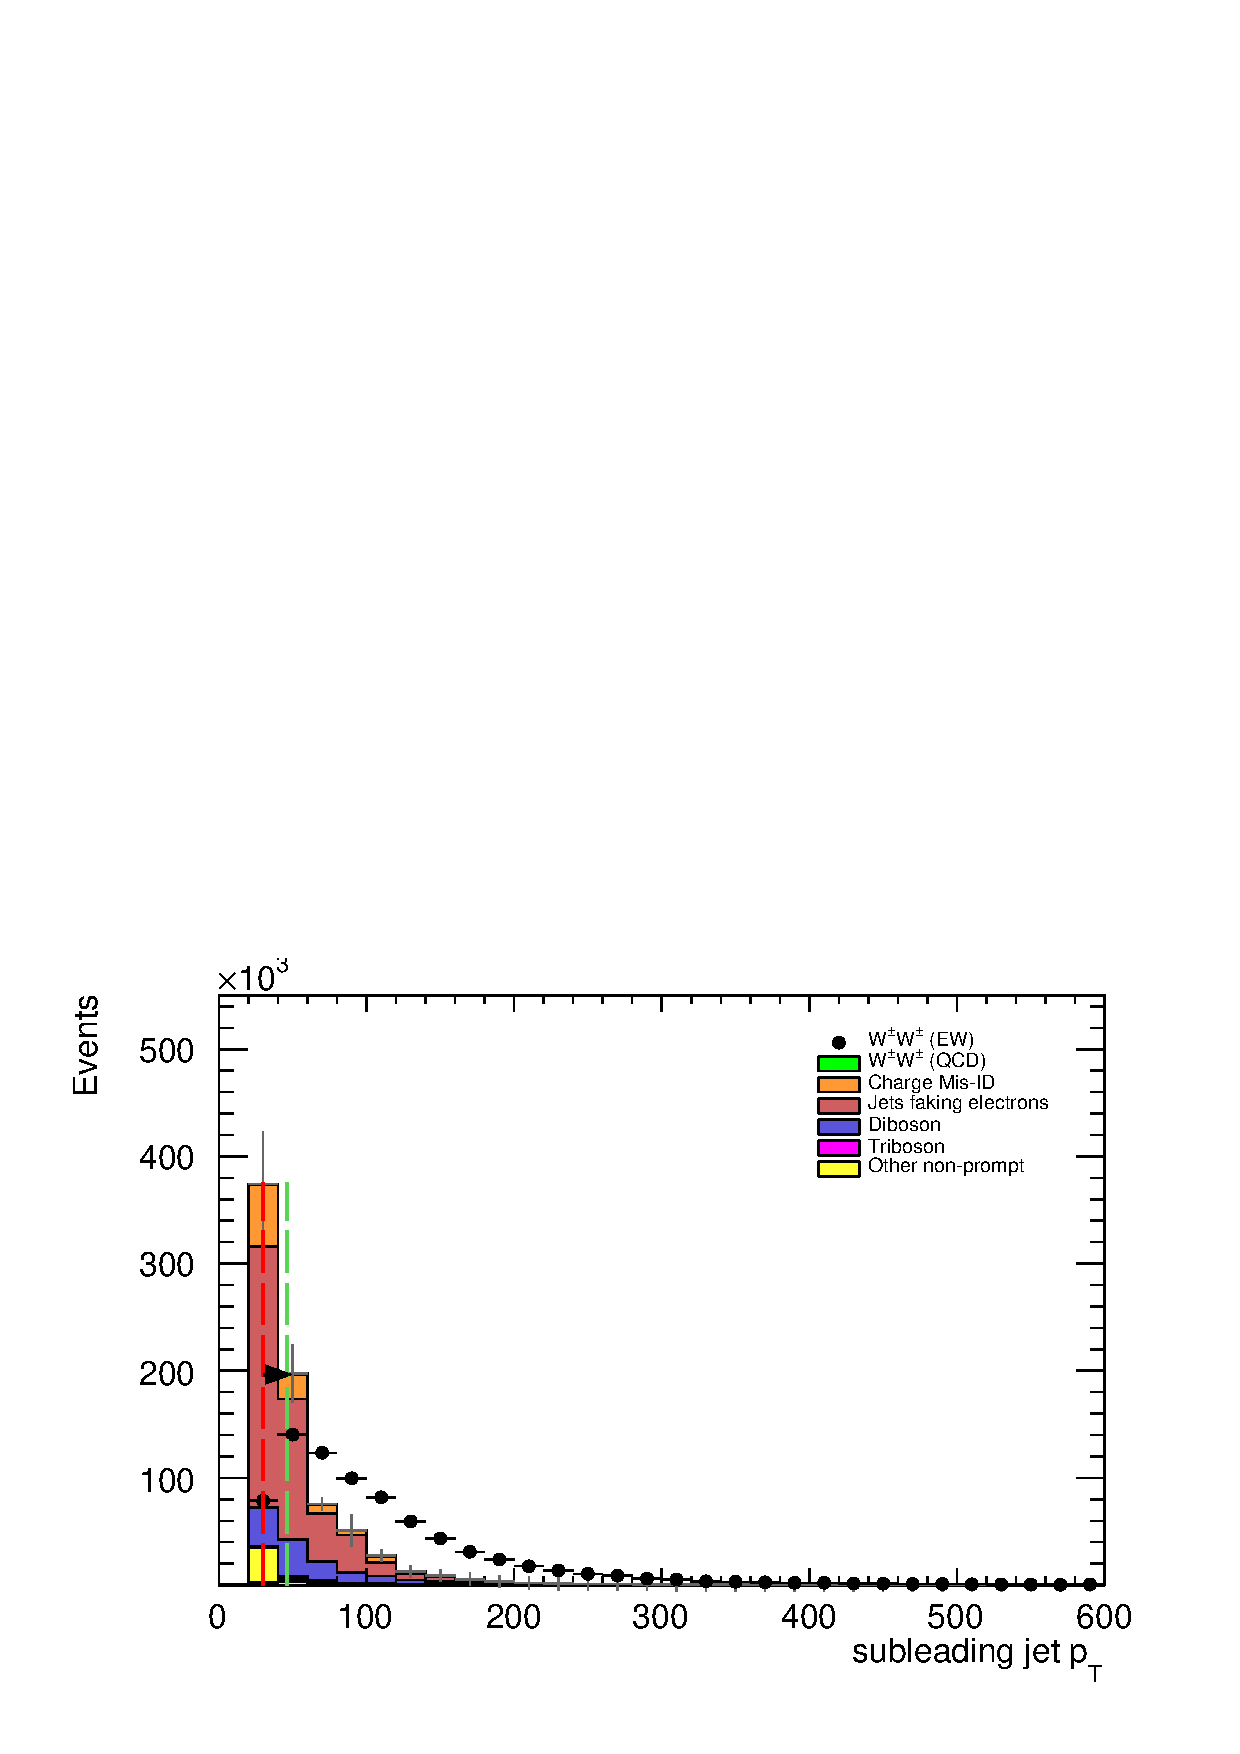
\includegraphics[width=0.6\textwidth]{figs/ssww_upgrade/optimization_plots/jet1pt}
  \caption{Leading (top) and subleading (bottom) jet $\pt$ distributions.  The default and optimized cuts are represented by the red and green dashed lines, respectively.  The \ssww EWK signal (black points) is normalized to the same area as the sum of the backgrounds (colored histogram).}
  \label{fig:optimized_jetpt}
\end{figure}

\begin{figure}[htp]
  \centering
  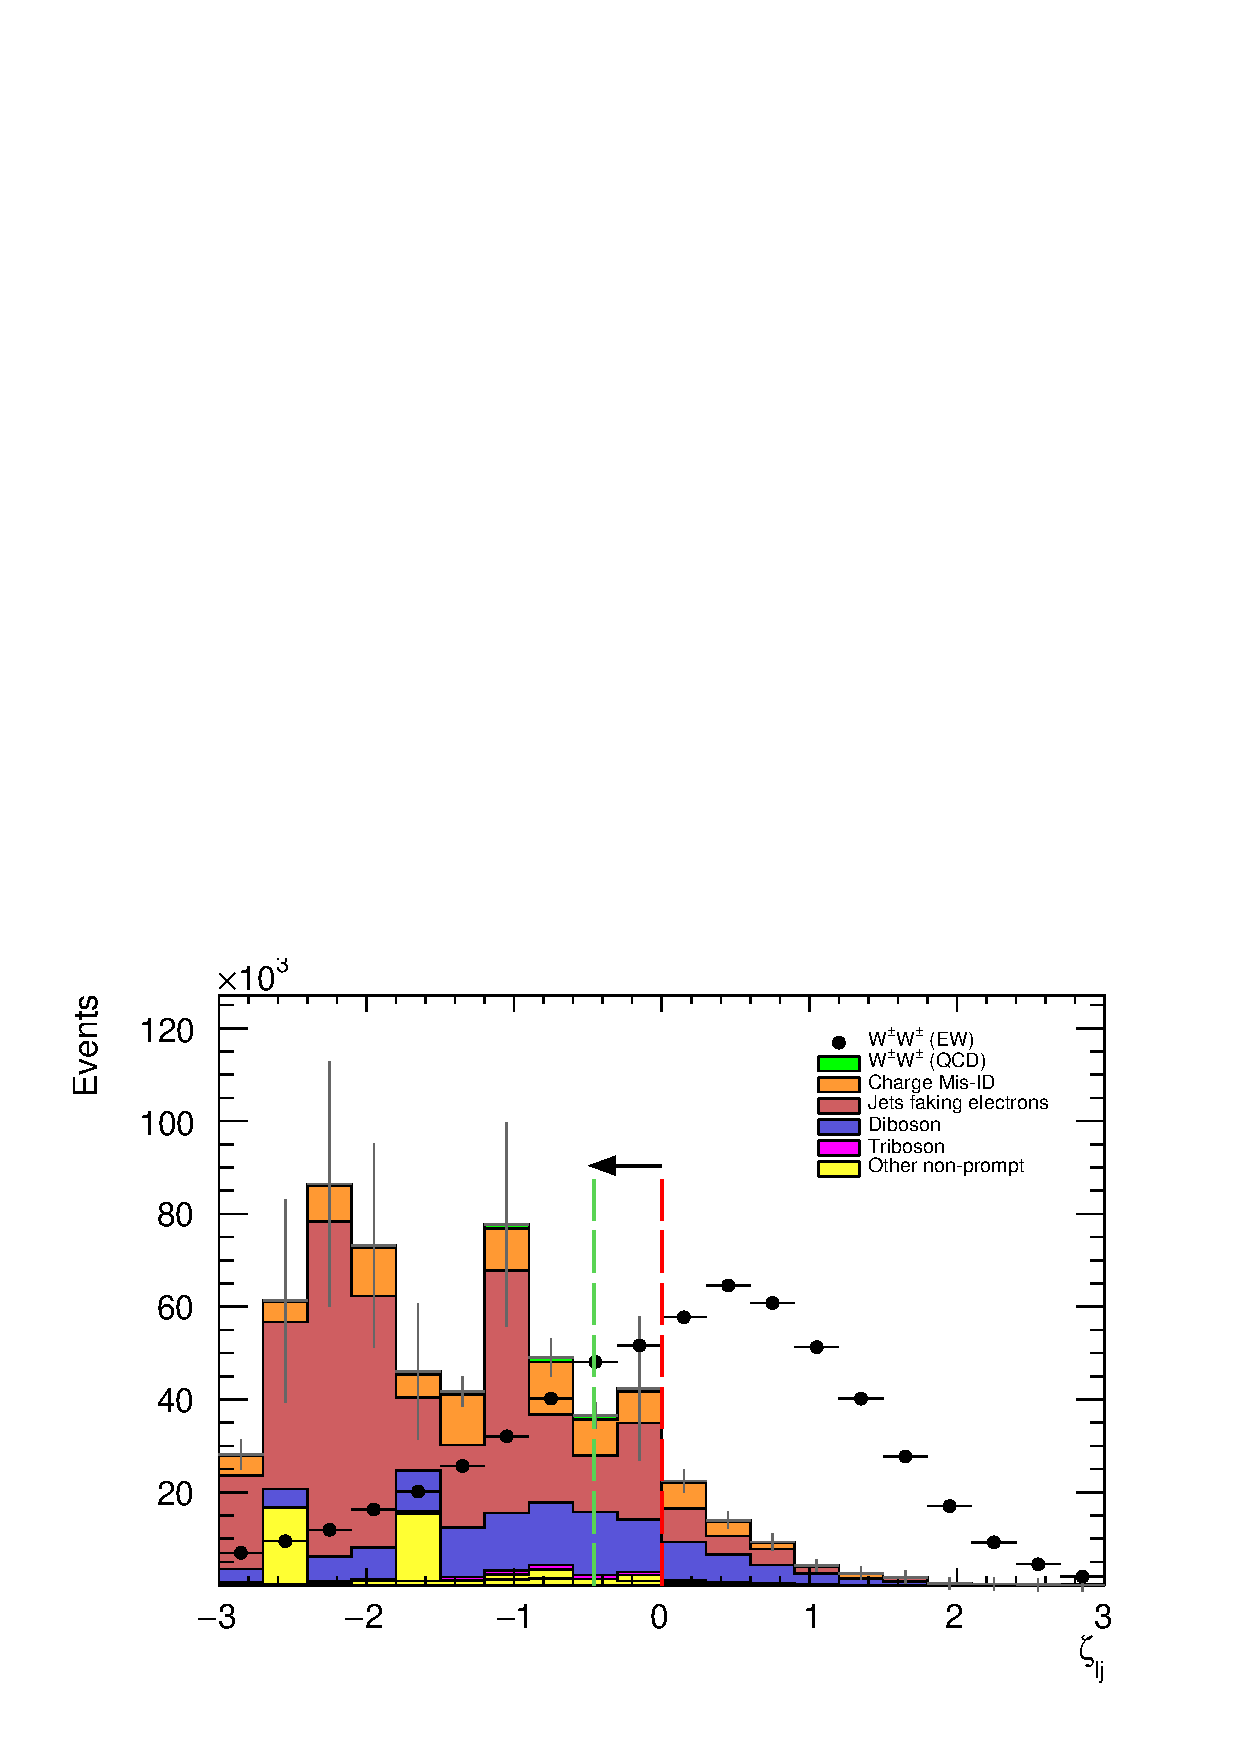
\includegraphics[width=0.6\textwidth]{figs/ssww_upgrade/optimization_plots/centrality}
  \caption{Lepton-jet centrality distribution.  The default and optimized cuts are represented by the red and green dashed lines, respectively.  The \ssww EWK signal (black points) is normalized to the same area as the sum of the backgrounds (colored histogram).}
  \label{fig:optimized_centrality}
\end{figure}
